\documentclass[a4paper, 12pt]{article}

%%% Работа с русским языком
\usepackage{cmap}					% поиск в PDF
\usepackage{mathtext} 				% русские буквы в формулах
\usepackage[T2A]{fontenc}			% кодировка
\usepackage[utf8]{inputenc}			% кодировка исходного текста
\usepackage[russian]{babel}	% локализация и переносы

%%% Дополнительная работа с математикой
\usepackage{amsmath,amsfonts,amssymb,amsthm,mathtools} % AMS
\usepackage{icomma} % "Умная" запятая: $0,2$ --- число, $0, 2$ --- перечисление

%% Номера формул
%\mathtoolsset{showonlyrefs=true} % Показывать номера только у тех формул, на которые есть \eqref{} в тексте.

%% Шрифты
\usepackage{euscript}	 % Шрифт Евклид
\usepackage{mathrsfs} % Красивый матшрифт

%% Поля
\usepackage[left=2cm,right=2cm,top=2cm,bottom=2cm,bindingoffset=0cm]{geometry}

%% Русские списки
\usepackage{enumitem}
\makeatletter
\AddEnumerateCounter{\asbuk}{\russian@alph}{щ}
\makeatother

%%% Работа с картинками
\usepackage{graphicx}  % Для вставки рисунков
\graphicspath{{images/}{images2/}}  % папки с картинками
\setlength\fboxsep{3pt} % Отступ рамки \fbox{} от рисунка
\setlength\fboxrule{1pt} % Толщина линий рамки \fbox{}
\usepackage{wrapfig} % Обтекание рисунков и таблиц текстом

%%% Работа с таблицами
\usepackage{array,tabularx,tabulary,booktabs} % Дополнительная работа с таблицами
\usepackage{longtable}  % Длинные таблицы
\usepackage{multirow} % Слияние строк в таблице

%% Красная строка
\setlength{\parindent}{2em}

%% Интервалы
\linespread{1}
\usepackage{multirow}

%% TikZ
\usepackage{tikz}
\usetikzlibrary{graphs,graphs.standard}

%% Верхний колонтитул
\usepackage{fancyhdr}
\pagestyle{fancy}

%% Перенос знаков в формулах (по Львовскому)
\newcommand*{\hm}[1]{#1\nobreak\discretionary{}
	{\hbox{$\mathsurround=0pt #1$}}{}}

%% Мои дополнения
\usepackage{float} %Добавляет возможность работы с командой [H] которая улучшает расположение на странице
\usepackage{gensymb} %Красивые градусы
\usepackage{graphicx}               % Импорт изображений
\usepackage{caption} % Пакет для подписей к рисункам, в частности, для работы caption*

% подключаем hyperref (для ссылок внутри  pdf)
\usepackage[unicode, pdftex]{hyperref}

%%% Теоремы
\theoremstyle{plain}                    % Это стиль по умолчанию, его можно не переопределять.
\renewcommand\qedsymbol{$\blacksquare$} % переопределение символа завершения доказательства

\newtheorem{theorem}{Теорема}[section] % Теорема (счетчик по секиям)
\newtheorem{proposition}{Утверждение}[section] % Утверждение (счетчик по секиям)
\newtheorem{definition}{Определение}[section] % Определение (счетчик по секиям)
\newtheorem{corollary}{Следствие}[theorem] % Следстиве (счетчик по теоремам)
\newtheorem{problem}{Задача}[section] % Задача (счетчик по секиям)
\newtheorem*{remark}{Примечание} % Примечание (можно переопределить, как Замечание)
\newtheorem{lemma}{Лемма}[section] % Лемма (счетчик по секиям)

\begin{document}
    \newcommand{\HRule}{\rule{\linewidth}{0.7mm}} % Defines a new command for the horizontal lines, change thickness here
	
	\begin{center}
		\large\textbf{Московский Физико-Технический Институт}\\ % Name of your university/college
		\large\textbf{(государственный университет)}
	
		\vfill
		
		\Large Лабораторная работа по курсу общей физики № *labnum*\\[0.5cm] % Preambule of your document title
		
		
		\HRule
		\\[0.4cm]
		{ \huge \bfseries *name of your labwork*}% Title of your document
		\\[0.4cm] 
		\HRule
		\\[0.5cm]
		
		\ \\
	\textbf{\large Автор:} \\	
	\large *your name* *groupname*\\ % Your name and something more, your group num for example
		\vfill
		\hspace*{-0.8 cm}
\includegraphics[width=100 pt]{frkt_logo}\\ % logo of your  company/university/college
		\large Долгопрудный, 2021 % location and year
	\end{center}

\newpage
\setcounter{page}{2}
\fancyfoot[c]{\thepage}
\fancyhead[L] {Работа № *labnum*} % some information in page header
\fancyhead[R]{}

    \section*{Цель работы}

    Снять и исследовать спектры излучения различных источников, характеризовать различные пики в спектрах радиоактивных веществ.

    \section*{Теоретическая чать}

    Основная задача спектрометрических измерений заключается в определении энергии, интенсивности дискретных гамма-линий от различных гамма-источников и их идентификации.
	
	Основными процессами взаимодействия гамма-излучения с веществом являются фотоэффект, эффект Комптона и образование электрон-позитронных пар. Каждый из этих процессов вносит свой вклад в образование наблюдаемого спектра. Образующиеся при этих процессах электроны испытывают большое количество неупругих соударений с молекулами и атомами среды. Неупругие соударения могут сопровождаться как ионизацией, так и возбуждением молекул или атомов среды. В промежуточных же стадиях (при переходах возбужденных молекул или атомов в основное состояние, при рекомбинации электрических зарядов и т.п.) в веществе возникают кванты света различных длин волн, присущих данному веществу.
	
	При \textbf{фотоэффекте} кинетическая энергия электрона $ T_e = E_{\gamma} - I_i $, где $ I_i $ --- энергия ионизации $ i $-той оболочки атома. Фотоэффект особенно существенен для тяжелых веществ, где он идет с заметной вероятностью даже при высоких энергиях гамма-квантов. В легких веществах фотоэффект становится заметен лишь при относительно небольших энергиях гамма-квантов. Наряду с фотоэффектом, при котором вся энергия гамма-кванта передается атомному электрону, взаимодействие гамма-излучения со средой может приводить к его рассеянию, т.е. отклонению от первоначального направления распространения на некоторый угол.
	
	При \textbf{эффекте Компотна} происходит упругое рассеяние фотона на свободном электроне, сопровождающееся изменением длины волны фотона (реально этот процесс происходит на слабо связанных с атомом внешних электронах). Максимальная энергия образующихся комптоновских электронов соответствует рассеянию гамма-квантов на $ 2\pi $ и равна
	
	\begin{equation}\label{E_compton}
	E_{с \_ max} = \dfrac{\hbar \omega}{1 + \dfrac{m_ec^2}{2\hbar\omega}}
	\end{equation}
	
	При достаточно высокой энергии гамма-кванта наряду с фотоэффектом и эффектом Комптона может происходить третий вид взаимодействия гамма-квантов с веществом – \textbf{образование электрон-позитронных пар}. При этом если процесс образования пары идет в кулоновском поле ядра или протона, то энергия образующегося ядра отдачи оказывается весьма малой, так что пороговая энергия гамма-кванта, необходимая для образования пары, практически совпадает с удвоенной энергией покоя электрона $ Е_0 = 2m_ec^2 =1,022  $МэВ.
	
	Появившийся в результате процесса образования пар электрон теряет свою энергию на ионизацию среды. Таким образом, вся энергия электрона остается в детекторе. Позитрон будет двигаться до тех пор, пока практически не остановится, а затем аннигилирует с электроном среды, в результате чего появятся два гамма-кванта. Т.е., кинетическая энергия позитрона также останется в детекторе. Далее возможны три варианта развития событий:
	
	а) оба родившихся гамма-кванта не вылетают из детектора, и тогда вся энергия первичного гамма-кванта останется в детекторе, а в спектре появится пик с $ E = E_\gamma $;
	
	б) один из родившихся гамма-квантов покидает детектор, и в спектре появляется пик, соответствующий энергии $  Е = Е_\gamma - E0 $, где $ Е_0 = m_ec^2 = $ 511 кэВ;
	
	в) оба родившихся гамма-кванта покидают детектор, и в спектре появля- ется пик, соответствующий энергии $  Е = Е_\gamma - 2E0 $, где $ 2Е_0 = 2m_ec^2 = $ 1022 кэВ;
	
	Таким образом, любой спектр, получаемый с помощью гамма-спектрометра, описывается несколькими компонентами, каждая из которых связана с определенным физическим процессом. Как описано выше, основными физическими процессами взаимодействия гамма-квантов с веществом являются фотоэффект, эффект Комптона и образование электрон-позитронных пар, и каждый из них вносит свой вклад в образование спектра. Помимо этих процессов, добавляются экспонента, связанная с наличием фона, пик характеристического излучения, возникающий при взаимодействии гамма-квантов с окружающим веществом, а также пик обратного рассеяния, образующийся при энергии квантов $ Е_\gamma \gg mc^22/2 $ в результате рассеяния гамма-квантов на большие углы на материалах конструктивных элементов детектора и защиты. Положение пика обратного рассеяния определяется по формуле ($ E $ --- энергия фотопика):
	
	\begin{equation}\label{Eobr}
		E_{обр} = \dfrac{E}{1 + \dfrac{2E}{mc^2}}
	\end{equation}

%	\section{Экспериментальная установка}
%	
	Энергетическим разрешением спектрометра называется величина
	
	\begin{equation}\label{Ri = dE/E}
	R_i = \dfrac{\Delta E_i}{E_i}
	\end{equation}
	
	т.е. отношение ширины пика полного поглощения (измеренной на полувысоте) к регистрируемой энергии пика поглощения. Это значение $ E_i \propto \overline{n_i} $ --- числу частиц на выходе ФЭУ. При этом  $ \Delta E_i \propto \overline{\Delta n_i} = \sqrt{\overline{n_i}} $ --- ширина пика пропорциональна среднеквадратичной флуктуации, которая равна корню из числа частиц. Таким образом, наша формула \eqref{Ri = dE/E} примет вид
	
	\begin{equation}\label{Ri = c/E}
	R_i = \dfrac{\mathrm{const}}{\sqrt{E_i}}
	\end{equation}

    \section*{Обработка эксперементальных данных}

	Снимем данные для образцов. По полученным данным построим графики (предварительно из каждого спектра
	вычтем спектр шума) рис \ref{fig:spectrum}.

	\begin{figure}
		\centering
		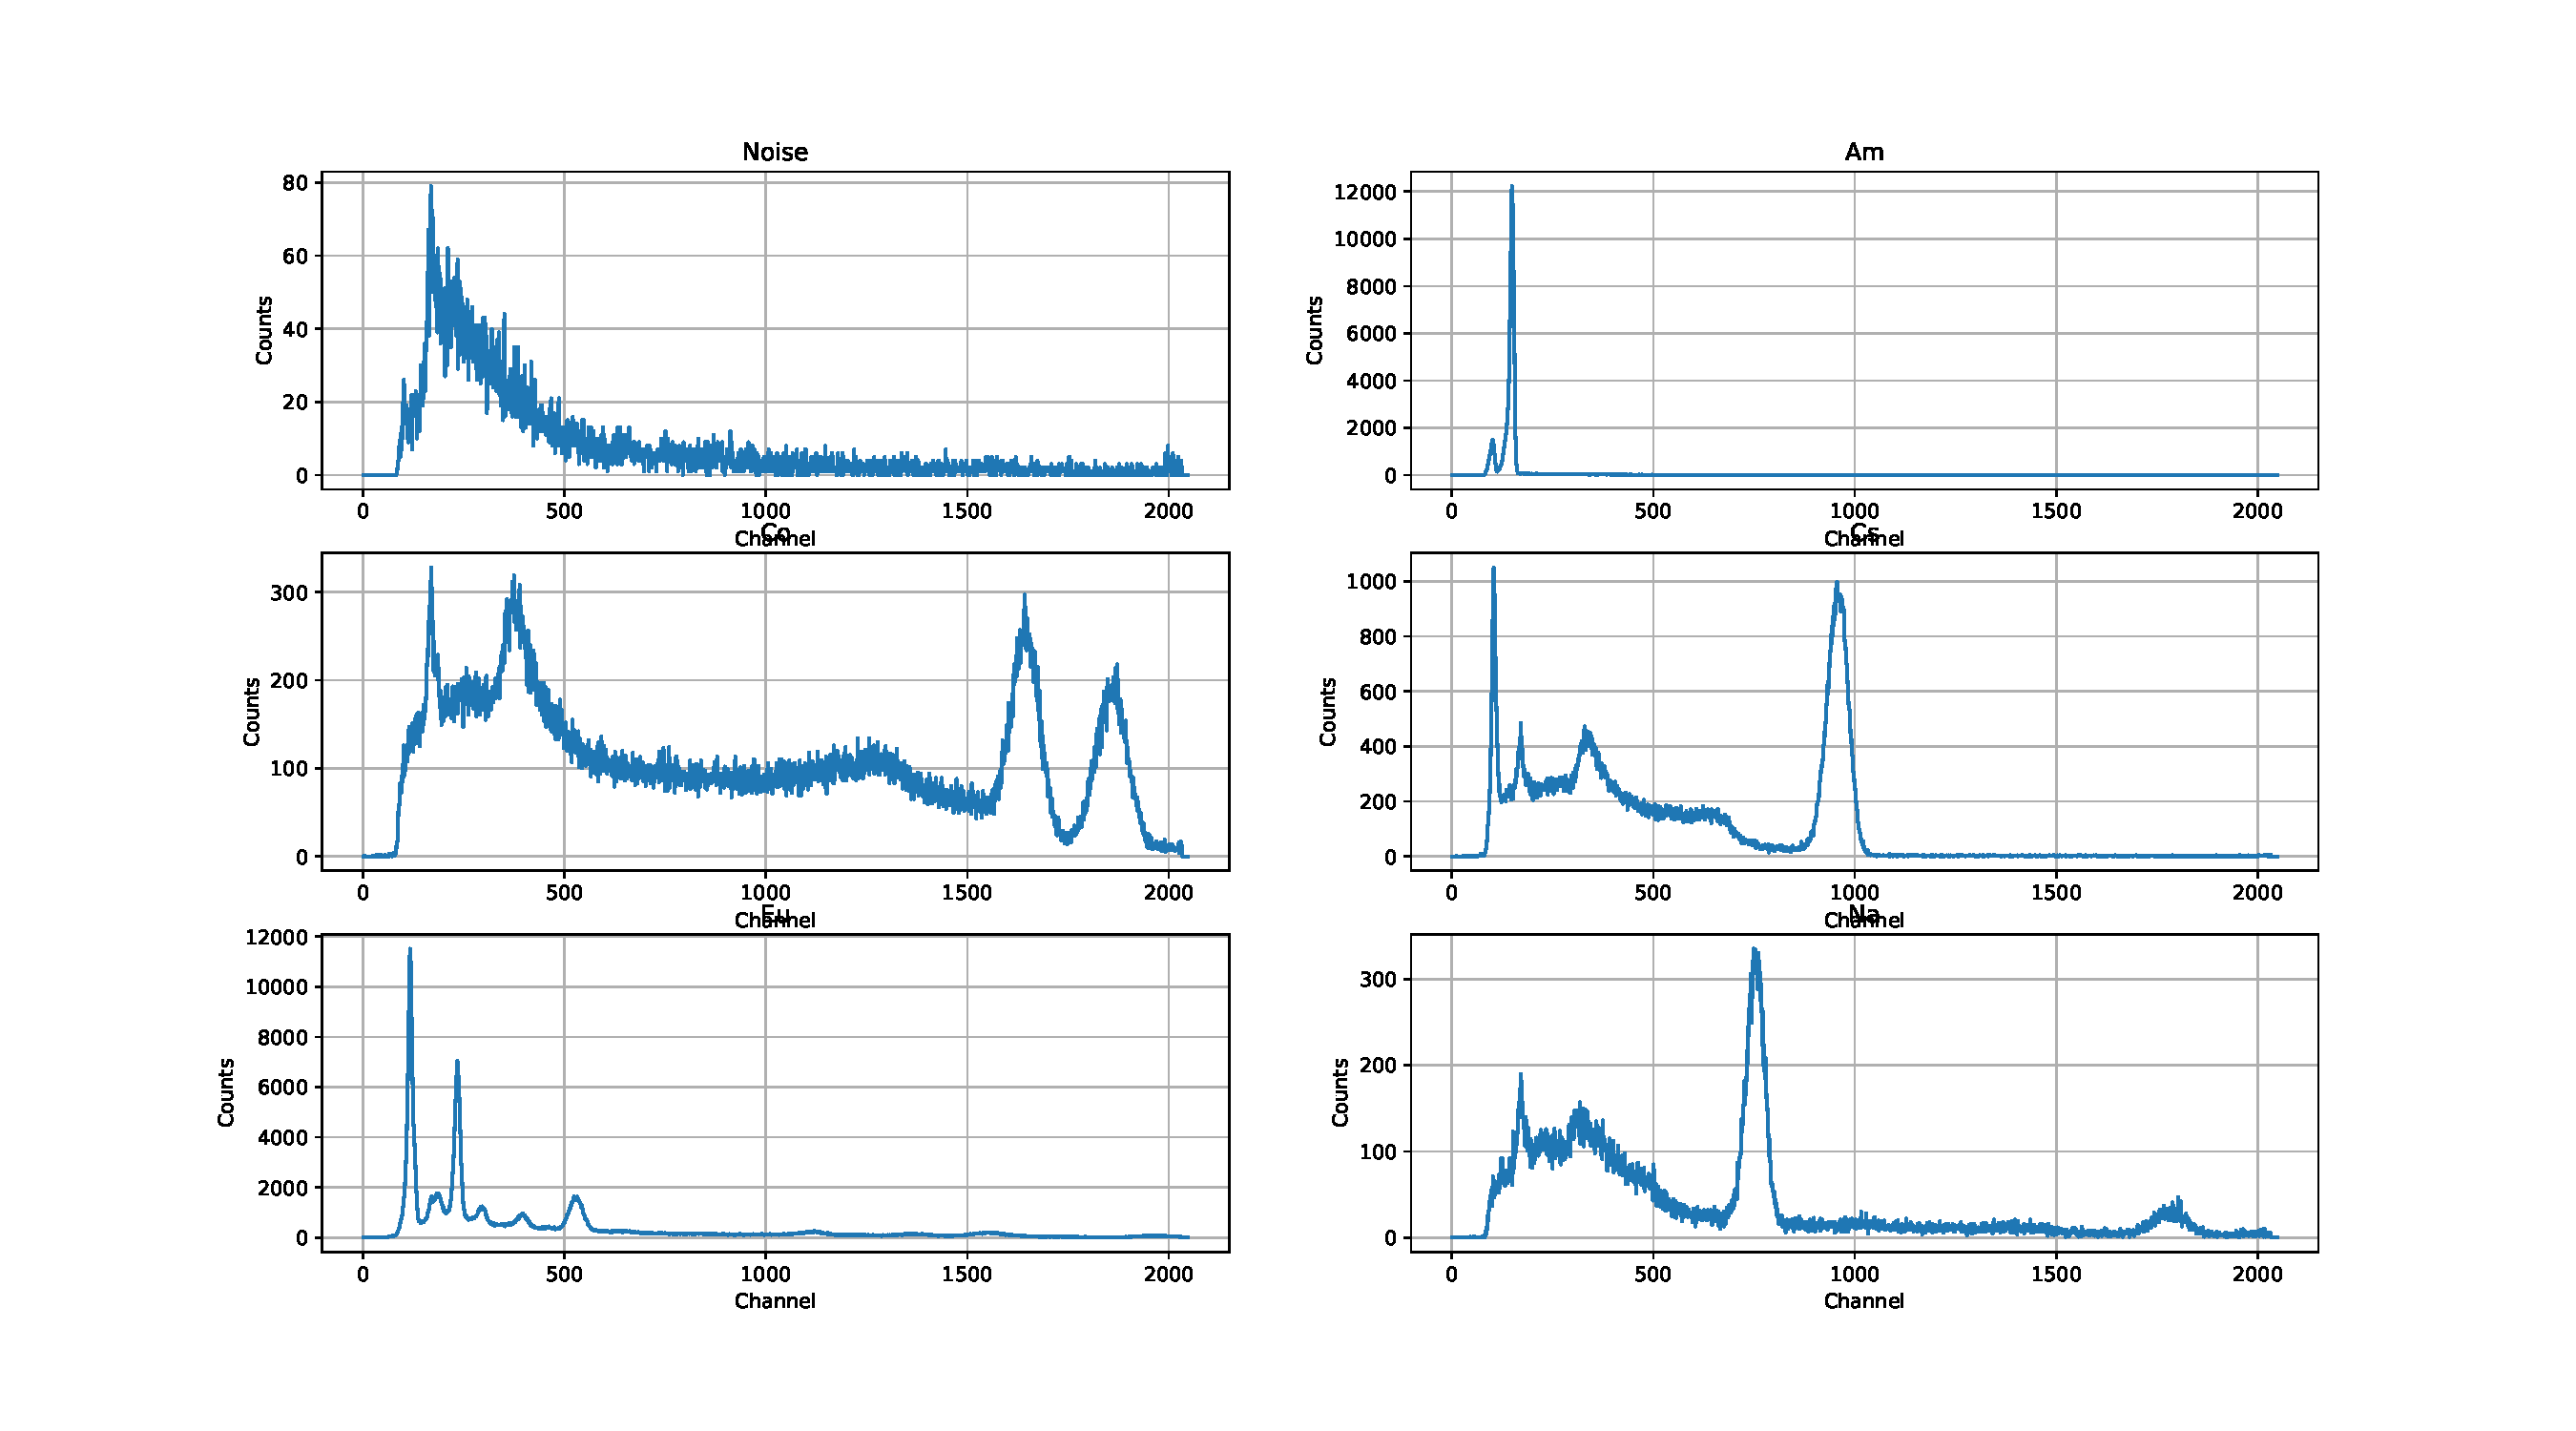
\includegraphics[width=\textwidth]{all_graphs.pdf}
		\caption{Спектры для всех элементов}
		\label{fig:spectrum}
	\end{figure}

	Используя известные (табличные) значения энергий пиков, соответствующих определенным каналам, найдем
	линейное преобразования номера канала в энергию пика рис \ref{fig:Channel2Energy}.

	\begin{figure}
		\centering
		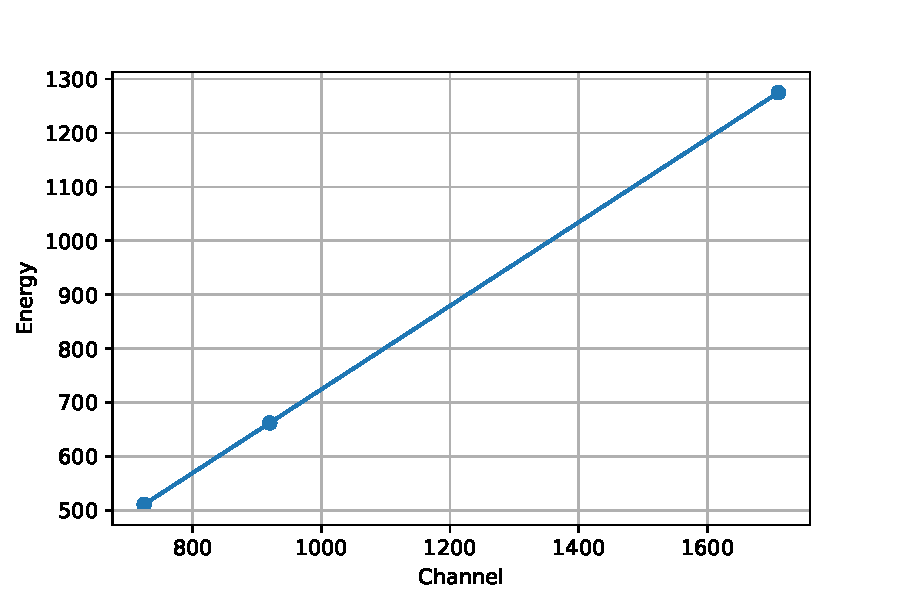
\includegraphics[width=\textwidth]{Channel2Energy.pdf}
		\caption{График перевода номера канала в значение энергии}
		\label{fig:Channel2Energy}
	\end{figure}

	Таким образом, линейное преобразование имеет вид

	\[ E = (-53.23 \pm 7.10) + (0.7469 \pm 0.006) N ~ [\text{кэВ}] \]

	\begin{center}
		Пики натрия: \\
		511 кэВ -- канал 725 \\
		1275 кэВ -- канал 1710 \\[1 cm]
		Пик цезия: \\
		662 кэВ -- канал 920
	\end{center}b

    % значению канала соответсвует значение энергии гамма-кванта
    % нам известны значения энергий фотопиков для 3х изотопов
    % эксперементально мы можем узнать номера каналов фотопиков для этих изотопов
    % поскольку зависимость линейная, мы можем построить линейный график и однозначно определять энергию по значению канала

	Используя полученное преобразование, найдем энергии пиков полного поглащения для всех остальных
	элементов \ref{tab:main_table}.

	\begin{table}[h!]
    \centering
    \begin{tabular}{|c|c|c|c|c|c|}
    \hline
    Элемент & $N$   & $\Delta N$ & $E$, кэВ  & $\Delta E$, кэВ & $R$    \\ \hline
    Na      & 1779  & 83         & 1281,02  & 62,25          & 0,049  \\ \hline
    Na      & 759   & 51         & 516,02   & 38,25          & 0,074  \\ \hline
    Co      & 1638  & 84         & 1175,27  & 63,00          & 0,054  \\ \hline
    Co      & 1856  & 88         & 1338,77  & 66,00          & 0,049  \\ \hline
    Cs      & 953   & 58         & 661,52   & 43,50          & 0,066  \\ \hline
    Am      & 149   & 10         & 58,52    & 7,50           & 0,128  \\ \hline
    Eu      & 524   & 38         & 339,77   & 28,50          & 0,084  \\ \hline
    Eu      & 394   & 25         & 242,27   & 18,75          & 0,077  \\ \hline
    Eu      & 294   & 25         & 167,27   & 18,75          & 0,112  \\ \hline
    \end{tabular}
    \caption{Энергии пиков полного поглащения}
    \label{tab:main_tab}
\end{table}

    Определим энергии края комптоновского поглощения для Co, Cs и Na, и сравним с теоретическими значениями \ref{tab:kompton}.

    \begin{table}[h!]
    \centering
    \begin{tabular}{|c|c|c|}
    \hline
       & exp  & thr  \\ \hline
    Co & 895  & 963  \\ \hline
    Cs & 425  & 477  \\ \hline
    Na & 1072 & 1062 \\ \hline
    \end{tabular}
    \caption{Край комптоновского рассеяния}
    \label{tab:kompton}
\end{table}

    Определим энергии пиков обратного рассеяния и сравним их с теоретическими \ref{tab:back_f}.

    \begin{table}[h!]
    \centering
    \begin{tabular}{|c|c|c|}
    \hline
       & exp & thr \\ \hline
    Co & 220 & 214 \\ \hline
    Cs & 197 & 184 \\ \hline
    \end{tabular}
    \caption{Энергии пиков обратного рассеяния}
    \label{tab:back_f}
\end{table}

	Построим график зависимости квадрата разрешения спектрометра для проверки формулы

	\[ R_i = \dfrac{\mathrm{const}}{\sqrt{E_i}} \]

	\begin{figure}
		\centering
		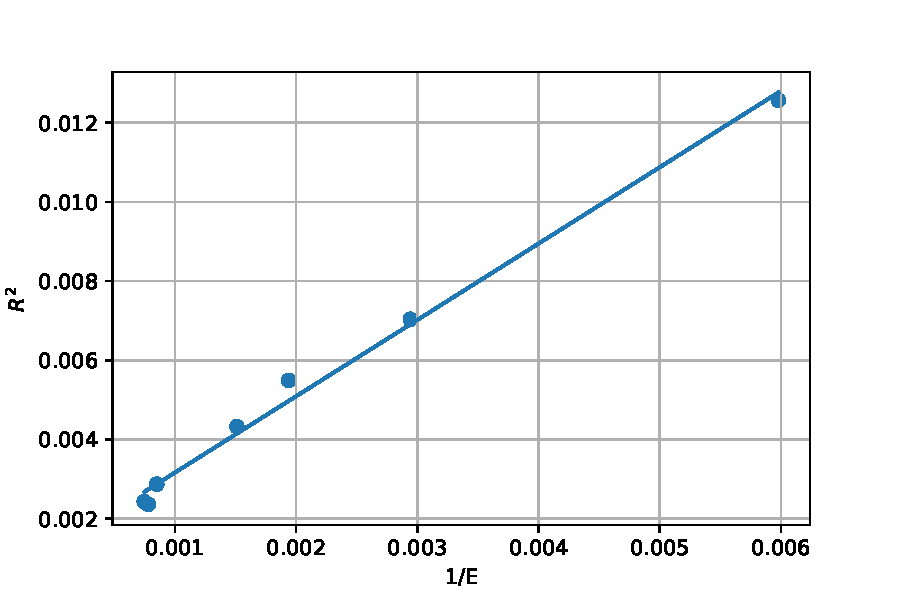
\includegraphics[scale=1]{R2.pdf}
		\caption{Проверка формулы $R_i = \dfrac{\mathrm{const}}{\sqrt{E_i}}$}
		\label{fig:R2}
	\end{figure}

	\begin{figure}
		\centering
		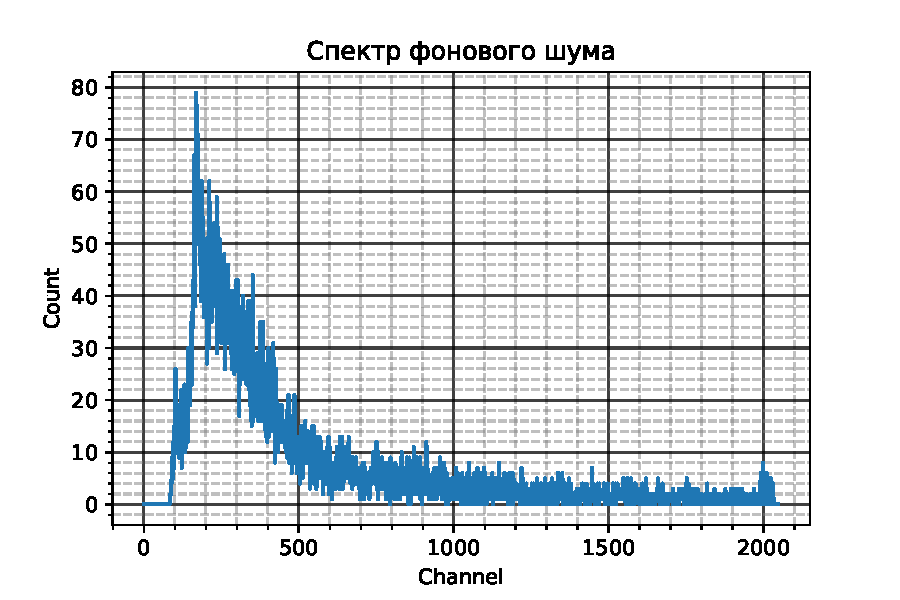
\includegraphics[width=\textwidth]{Noise.pdf}
		\caption{Спектры для всех элементов}
		\label{fig:Noise}
	\end{figure}

	\begin{figure}
		\centering
		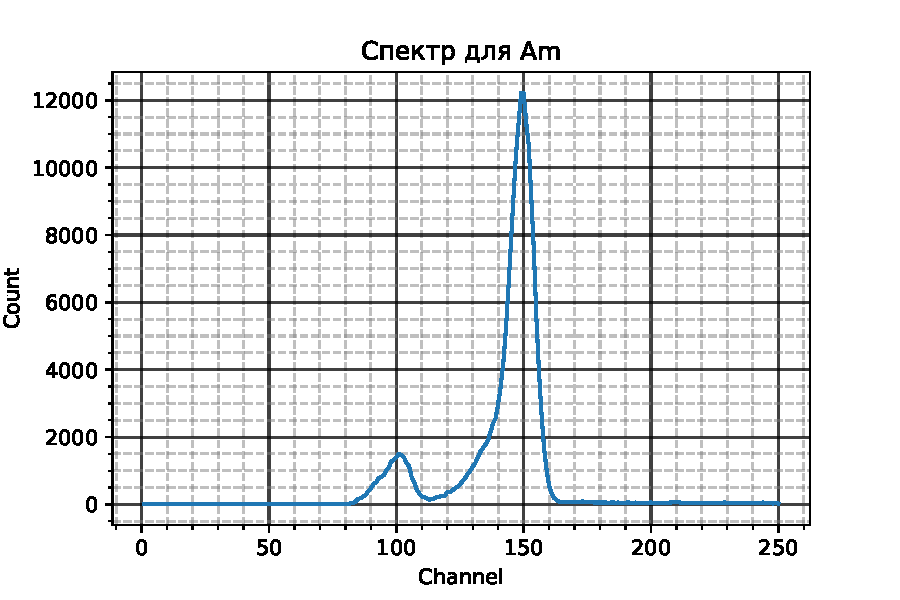
\includegraphics[width=\textwidth]{Am.pdf}
		\caption{Спектры для всех элементов}
		\label{fig:Am}
	\end{figure}

	\begin{figure}
		\centering
		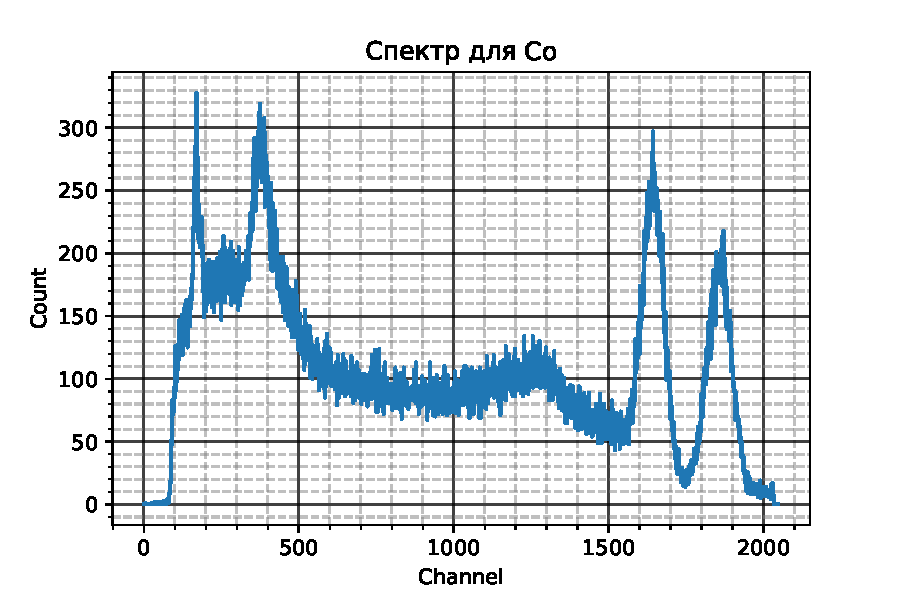
\includegraphics[width=\textwidth]{Co.pdf}
		\caption{Спектры для всех элементов}
		\label{fig:Co}
	\end{figure}

	\begin{figure}
		\centering
		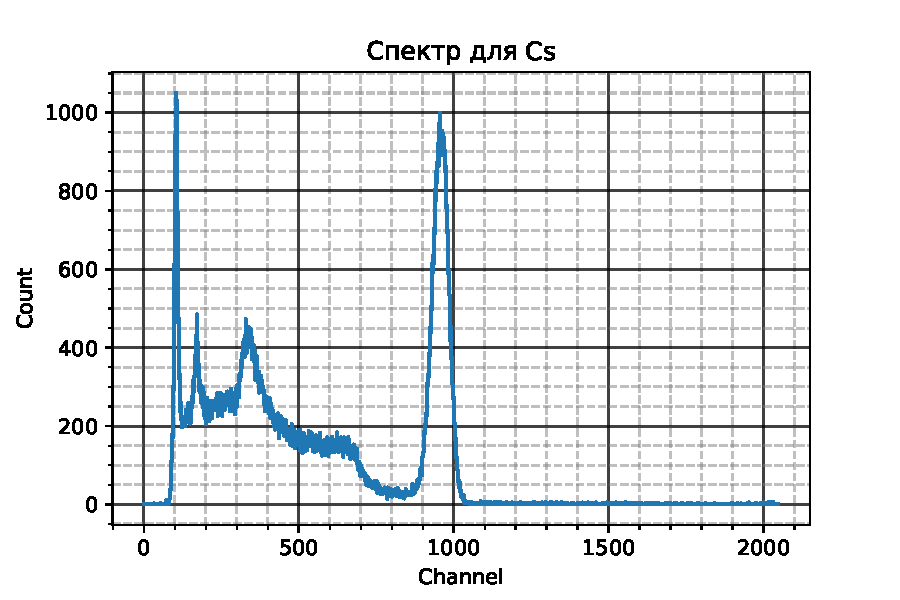
\includegraphics[width=\textwidth]{Cs.pdf}
		\caption{Спектры для всех элементов}
		\label{fig:Cs}
	\end{figure}

	\begin{figure}
		\centering
		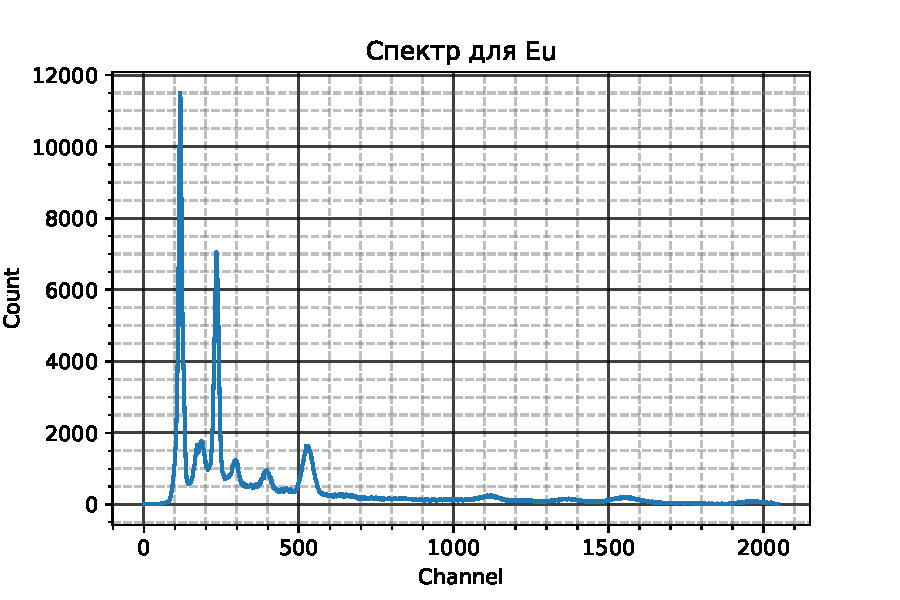
\includegraphics[width=\textwidth]{Eu.pdf}
		\caption{Спектры для всех элементов}
		\label{fig:Eu}
	\end{figure}

	\begin{figure}
		\centering
		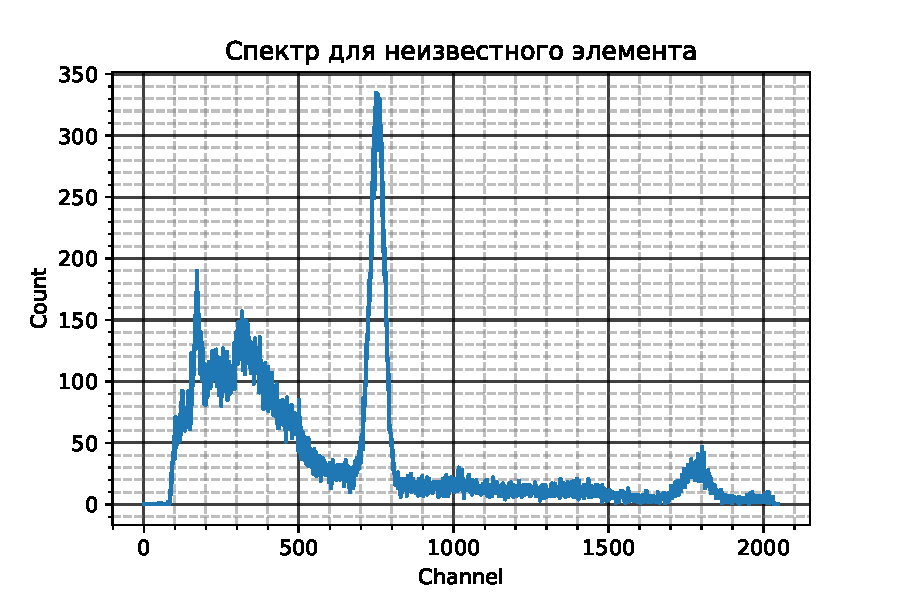
\includegraphics[width=\textwidth]{Na.pdf}
		\caption{Спектры для всех элементов}
		\label{fig:Na}
	\end{figure}



	\section*{Вывод}

	В ходе работы после калибровки прибора были сняты спектры образцов $^{22}$Na,  $^{60}$Cо,  $^{137}$Cs, $^{241}$Am, $^{152}$Eu, а также исследован спектр неизвестного образца и определен его состав ($^{137}$Cs). В спектрах были исследованы пики, соответствующие следующим взаимодействиям гамма-квантов с веществом:
	\begin{itemize}
		\item фотоэффект (пики полного поглощения)
		\item эффект Комптона (характерное распределение энергий в спектре, оканчивающееся комптоновским краем)
		\item обратное рассеяние (пики обратного рассеяния)
		\item аннигиляция позитронов (пик 511 keV в спектре натрия, по которому проводилась калибровка)
	\end{itemize}

	Все значения энергии, опеределённые по спектрам, практически совпадали с табличными и расчётными. \par

	Также была проверена линейная зависимость квадрата спектрального разрешения прибора от величины, обратной энергии полного поглощения.


\end{document}